\scanpage{48}
% E: text|upper left date|7.2.1984
\unsure{7.2.1984}
% E: text|upper left heading and paragraph|Structure de K
\uline{Structure de \(K\)}. \unsure{En y portant} des sommets d'ordre 2, soit \(S_K\) l'ens des sommets. On désigne par \(K\) le graphe top. \unsure{avec ces nouveaux sommets} (les anciens sont ceux de l'ordre 4). On a
% E: display|upper left, partition of vertices|S_K = S'_K union S''_K
\[
S_K=\underbrace{S'_K}_{\text{sommets rouges}}\sqcup
\underbrace{S''_K}_{\substack{\text{sommets}\ \deleted{\text{\unsure{rouges}}}\inserted{\text{noirs}}}}
\]
\margin{\uline{NB} \deleted{\unsure{\(S'_K\), \(S''_K\) sont}}\inserted{\(S'_K\) contient des} sommets d'ordre 2, \unsure{pas néc.|puis aussi} des sommets d'ordre 4. \(S''_K\) contient des sommets d'ordre 2, pas \unsure{néc.} d'ordre 4.}

% E: text|left middle, a|avec a) Pour tte face
avec :

a) Pour tte \deleted{\unsure{une}} face \(F\), \(S'_K\cap F\) et \(S''_K\cap F\) sont des subdivisions de \(\unsure{\delta F}\) \unsure{duales|doubles} l'une de l'autre, d'ordre \(2n\).

% E: text|left middle, NB|Deux sommets consécutifs
\deleted{\unsure{b)}}\inserted{NB} --- Deux sommets consécutifs sur \(\delta F\) ne sont pas d'ordre 4, et plus précisément, \deleted{entre deux} sur un arc de \(\delta F\) joignant deux sommets d'ordre 4, il y a toujours au moins un sommet rouge d'ordre 2, (et $=$ deux si \(\Sigma\) n'est pas \deleted{\unsure{double}} de type \(\mathrm{II}_p\) et si on est sur une arête exceptionnelle) et au moins un sommet noir (\unsure{il n'en est}\unsure{bq} pas dans le cas qu'on vient de dire\dots)

% E: text|lower left, b|On a une sélection
b) \deleted{\unsure{Enfin}} On a une \unsure{sélection des faces des bords} pour le déploiement \(K'\) de \(K\). Ainsi, chaque arête \(a\) d'une face \inserted{\(F\)} est munie d'un signe \(\varepsilon_F(a)\) qui est \(\unsure{+1|\pm1}\) si le bord est du côté de \(F\), \(-1\) sinon : On a les règles

% E: display|right upper, three sign rules|epsilon_F(a)
\[
\left\{\begin{array}{ll}
\varepsilon_F(a)=-\varepsilon_{F'}(a)&\text{si \(F,F'\) sont les deux faces incidentes à \(a\)}\\[6pt]
\varepsilon_F(\unsure{a})=\varepsilon_F(\unsure{b})&\begin{array}{l}\text{si \(a\) et \(b\) sont adjacentes}\\\text{sur \(F\), le sommet commun étant}\\\text{d'ordre 2}\end{array}\\[6pt]
\varepsilon_{a_1}(F_1)=\varepsilon_{a_2}(F_2)&\begin{array}{l}\text{si \(F_1\) et \(F_2\) sont adjacentes le long d'une}\\\text{arête quelconque \(b\), d'extrémité \(s\), d'ordre 4}\\\text{et que \(a_1\) et \(a_2\) sont incidentes à \(F_1\) et \(F_2\)}\\\text{resp., autres que \(b\), et incidentes à \(s\).}\end{array}
\end{array}\right.
\]
% E: drawing|right upper-middle below sign rules|b s cross
\figure{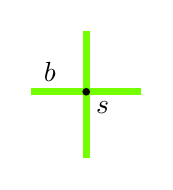
\begin{tikzpicture}[scale=.7]
\draw[green!55!yellow,line width=2.5pt](-1,0)--(1,0);\draw[green!55!yellow,line width=2.5pt](0,-1.2)--(0,1.1);
\fill(0,0)circle(2pt);\node[above]at(-.66,0){\(b\)};\node[below right]at(0,0){\(s\)};
\end{tikzpicture}}

% E: text|right middle, consequence|Il résulte du fait
Il résulte du fait que ttes les faces sont du $=$ ordre \(4n\), que pour \deleted{\unsure{chacune}} toute arête \(a\), si \(F,F'\) sont les deux faces incidentes, on a une donnée de \uline{symétrie autour de \(a\)}
% E: diagram|right middle, polygon isomorphism|sigma_a Pol(F) Pol(F')
\diagram{\begin{tikzcd}
\sigma_a^F\unsure{\simeq}\sigma_a:\ \deleted{\unsure{P}}\operatorname{Pol}(F)\arrow[r,"\sim"]&\operatorname{Pol}(F')
\end{tikzcd}}
\margin{\uline{NB} On a \(\sigma_a^F\sigma_a^{F'}=\mathrm{id}\).}
% E: text|right lower, characterization|caractérisé par la condition
\unsure{caractérisé par la condition de laisser} \deleted{invariantes}\inserted{fixes} les deux extrémités de \(a\). Il laisse donc \deleted{invariants}\inserted{fixes} \deleted{\unsure{tous}} tous les sommets et arêtes qui sont sur le ``grand côté'' \(\widehat a\) contenant \(a\) (bordé par les sommets d'ordre 4 les plus proches) (mais \deleted{\unsure{pas tous les pts}}\inserted{les prochains sommets} de part et d'autre de \(\widehat a\) sont non fixés par \(\sigma_a\)). L'application \(\sigma_a\) transforme sommets rouges (resp. noirs) en sommets noirs
\margin{\uline{NB} \(\sigma_a^F=\unsure{\sigma_{a'}^F|\sigma_a^{F'}}\) \unsure{si \(a,a'\) sont sur le $=$} \uline{\unsure{gd côté}}.}
\mspage{47}
